\documentclass[doublespacing]{bmcart}

%%% Load packages
\usepackage{amsthm,amsmath}
\RequirePackage{hyperref}
\usepackage[applemac]{inputenc} %applemac support if unicode package fails
%\usepackage[latin1]{inputenc} %UNIX support if unicode package fails
\usepackage{subcaption}


\def\includegraphic{}
\def\includegraphics{}


\usepackage{todonotes}
\usepackage{multirow}
%%% Put your definitions there:
\startlocaldefs
\newcommand{\pv}{\textit{P. vivax}}
\newcommand{\pf}{\textit{P. falciparum}}
\newcommand{\males}{M15$+$}
\graphicspath{{../figures/}}
\endlocaldefs


%%% Begin ...
\begin{document}

%%% Start of article front matter
\textbf{Supplemental appendix\: Assessing a 2020--2025 primaquine intervention in Cambodia to control vivax malaria}

\section*{Model structure}
\todo[inline]{details on the full model structure, parameter values, and calibration are provided in Additional file}
Table with default parameter values here, copy from Scott 2017 mostly

\section*{Data inputs}
\todo[inline]{Data on annual incidence (2011--2018), testing numbers, and demographics were used to calibrate the model for each population stratification (i.e. males 15 years and over, and everyone else) and province}
Table(s) with aggregated input values for each province

\section*{Calibrations}

\todo[inline]{Calibration values table: The model was calibrated to the incidence and test data using parameters for the relative susceptibility of the population group to malaria infection; the probability of developing malaria-like symptoms for each person in a given year; the daily probability of testing for people with non-severe malaria-like symptoms such as fever; the daily probability of testing for people with severe malaria-like symptoms; the duration of the latent period (i.e. until hypnozoite reactivation); the proportion incompletely clearing hypnozoites after naturally recovering; and the proportion of new malaria cases that are asymptomatic}

\begin{figure}[h]
\centering
\subcaptionbox{M15+, high.\label{Pursat_high_Incident_M15+}}{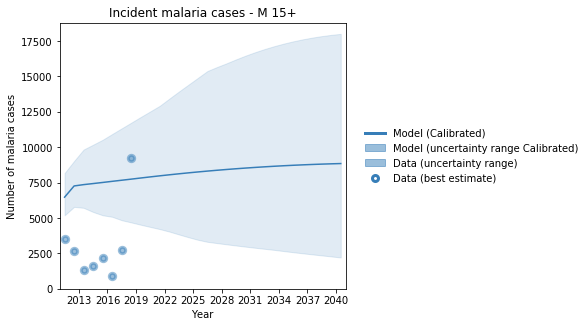
\includegraphics[width=.45\linewidth]{Pursat_high_Incident_M15+.png}} 
\subcaptionbox{Gen, high.\label{Pursat_high_Incident_Gen}}{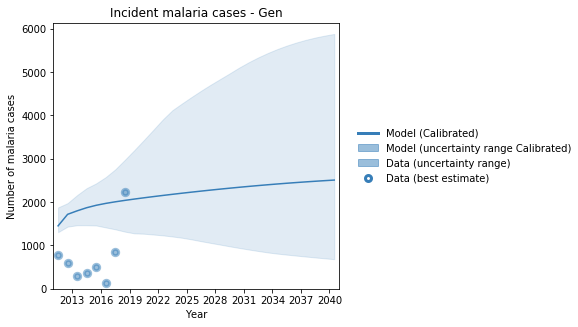
\includegraphics[width=.45\linewidth]{Pursat_high_Incident_Gen.png}} 
\subcaptionbox{M15+, low.\label{Pursat_low_Incident_M15+}}{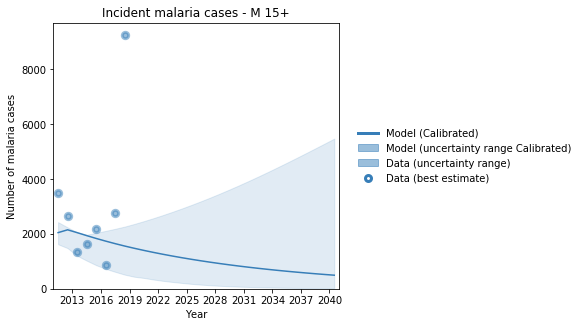
\includegraphics[width=.45\linewidth]{Pursat_low_Incident_M15+.png}} 
\subcaptionbox{Gen, low.\label{Pursat_low_Incident_Gen}}{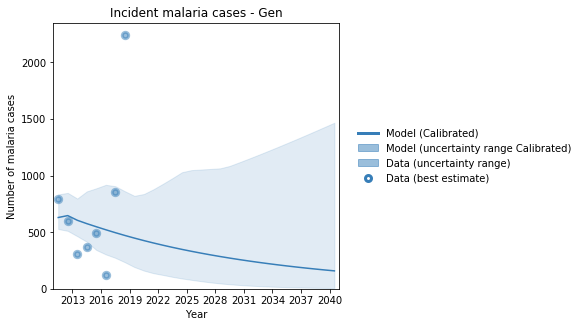
\includegraphics[width=.45\linewidth]{Pursat_low_Incident_Gen.png}} 
\caption{\csentence{Model calibration for Pursat.}}\label{fig:calibration_Pursat}
\end{figure}

\todo[inline]{Calibration plots as for Pursat to incident malaria cases for 5 other provinces}

\todo[inline]{The breakdown by state between latent and other stages of malaria (?)}

\section{Model outputs}
\todo[inline]{Tables of key outputs in each region? e.g. deaths as well as incidence?}

\end{document}
